\section*{Aufgabe 4: Testen von Grenzwerten und speziellen Werten}

\begin{lstlisting}[style=javastyle, caption=1.1: Tests]
[...]
public class NumberUtilsTest {
    NumberUtils numberUtils;

    @BeforeEach
    public void setUp() {
        this.numberUtils = new NumberUtils();
    }

    @Test
    public void testSumPositiveOnlyPositiveValues() {
        List<Integer> numbers = List.of(1, 2, 3, 4, 5);
        int result = numberUtils.sumPositive(numbers);
        assertEquals(15, result);
    }

    @Test
    public void testSumPositiveOnlyNegativeValues() {
        List<Integer> numbers = List.of(-1, -2, -3, -4, -5);
        int result = numberUtils.sumPositive(numbers);
        assertEquals(0, result);
    }

    @Test
    public void testSumPositiveMixedValues() {
        List<Integer> numbers = List.of(1, -1, 2, -2, 3, -3);
        int result = numberUtils.sumPositive(numbers);
        assertEquals(6, result);
    }

    // boundary cases:
    @Test
    public void testSumPositiveOnEmptyList() {
        List<Integer> numbers = List.of();
        int result = numberUtils.sumPositive(numbers);
        assertEquals(0, result);
    }

    @Test
    public void testSumPositiveOnSizeOneList() {
        List<Integer> numbers = List.of(1);
        int result = numberUtils.sumPositive(numbers);
        assertEquals(1, result);
    }

    @Test
    public void testSumPositiveOnSizeOneListNegativeValue() {
        List<Integer> numbers = List.of(-1);
        int result = numberUtils.sumPositive(numbers);
        assertEquals(0, result);
    }

    // edge cases:
    @Test
    public void testSumPositiveNull() {
        int result = numberUtils.sumPositive(null);
        assertEquals(0, result);
    }

    @Test
    public void testSumPositiveOnListWithZeroes() {
        List<Integer> numbers = List.of(0, 0, 0);
        int result = numberUtils.sumPositive(numbers);
        assertEquals(0, result);
    }

    @Test
    public void testSumPositiveOnNullList() {
        List<Integer> numbers = Arrays.asList(null, null, null);
        int result = numberUtils.sumPositive(numbers);
        assertEquals(0, result);

        numbers = Arrays.asList(null, null, null, 2, 4);
        result = numberUtils.sumPositive(numbers);
        assertEquals(6, result);
    }

    @Test
    public void testSumPositiveWithIntMaxValue() {
        List<Integer> numbers = List.of(Integer.MAX_VALUE, 1);
        int result = numberUtils.sumPositive(numbers);
        assertEquals(Integer.MIN_VALUE, result); // expecting overflow to Integer.MIN_VALUE
    }
}
\end{lstlisting}

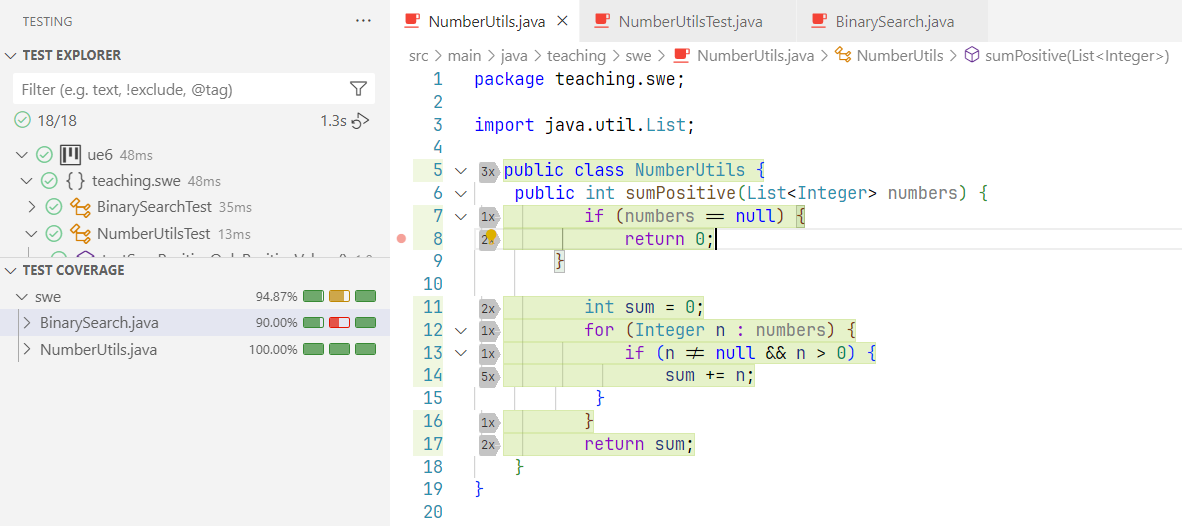
\includegraphics[width=\textwidth]{images/UE6_4.png}